\section{Introduction}

\begin{frame}{What is PGF/\TikZ?}
    \begin{itemize}
        \item Author: Till Tantau (University of L{\" u}beck)
        \item PGF: “Portable Graphics Format” (backend)
        \item \TikZ: “\TikZ ist \emph{kein} Zeichenprogramm” (frontend) (German for "\TikZ is \emph{not} a drawing program")
        \item Current version: 3.1.9a, \emph{1321 page manual}, {\scriptsize\url{https://pgf-tikz.github.io/pgf/pgfmanual.pdf}}
    \end{itemize}
\end{frame}

\section{Showcase}

\begin{frame}{Showcase - Example \#1}
    \begin{figure}
        \centering
        \begin{subfigure}[c]{0.3\textwidth}
            \centering
            \begin{adjustbox}{width=0.98\textwidth}
                % Rotated polygons
% Author: Dr. rer. nat. Ismael Gutierrez Garcia

\setcounter{density}{20}

\begin{tikzpicture}
    \def\couleur{BlueGreen}
    \path[coordinate] (0,0)  coordinate(A)
                ++( 120:6cm) coordinate(B)
                ++(60:6cm) coordinate(C)
                ++(0:6cm) coordinate(D)
                ++(-60:6cm) coordinate(E)
                ++(240:6cm) coordinate(F)
                ;
    \draw[fill=\couleur!\thedensity] (A) -- (B) -- (C) --(D) -- (E) -- (F)-- cycle;
    \foreach \x in {1,...,40}{%
        \pgfmathsetcounter{density}{\thedensity+10}
        \setcounter{density}{\thedensity}
        \path[coordinate] coordinate(X) at (A){};
        \path[coordinate] (A) -- (B) coordinate[pos=.10](A)
                            -- (C) coordinate[pos=.10](B)
                            -- (D) coordinate[pos=.10](C)
                            -- (E) coordinate[pos=.10](D)
                             -- (F) coordinate[pos=.10](E)
                            -- (X) coordinate[pos=.10](F);
        \draw[fill=\couleur!\thedensity] (A)--(B)--(C)-- (D) --(E) -- (F) -- cycle;
    }
\end{tikzpicture}
            \end{adjustbox}
        \end{subfigure}
        \begin{subfigure}[c]{0.3\textwidth}
            \centering
            \begin{adjustbox}{width=0.98\textwidth}
                % Rotated polygons
% Author: Dr. rer. nat. Ismael Gutierrez Garcia

\setcounter{density}{20}
\begin{tikzpicture}
    \def\couleur{LimeGreen}
    \path[coordinate] (0,0)  coordinate(A)
                ++( 144:10cm) coordinate(B)
                ++(72:10cm) coordinate(C)
                ++(0:10cm) coordinate(D)
                ++(-72:10cm) coordinate(E)
                                ;
    \draw[fill=\couleur!\thedensity] (A) -- (B) -- (C) --(D) -- (E) --  cycle;
    \foreach \x in {1,...,40}{%
        \pgfmathsetcounter{density}{\thedensity+10}
        \setcounter{density}{\thedensity}
        \path[coordinate] coordinate(X) at (A){};
        \path[coordinate] (A) -- (B) coordinate[pos=.10](A)
                            -- (C) coordinate[pos=.10](B)
                            -- (D) coordinate[pos=.10](C)
                            -- (E) coordinate[pos=.10](D)
                             -- (X) coordinate[pos=.10](E);
        \draw[fill=\couleur!\thedensity] (A)--(B)--(C)-- (D) --(E)  -- cycle;
    }
\end{tikzpicture}
            \end{adjustbox}
        \end{subfigure}
        \begin{subfigure}[c]{0.3\textwidth}
            \centering
            \begin{adjustbox}{width=0.98\textwidth}
                % Rotated polygons
% Author: Dr. rer. nat. Ismael Gutierrez Garcia

\setcounter{density}{20}
\begin{tikzpicture}
    \def\couleur{OrangeRed}
    \path[coordinate] (0,0)  coordinate(A)
                ++( 90:12cm) coordinate(B)
                ++(0:12cm) coordinate(C)
                ++(-90:12cm) coordinate(D);
    \draw[fill=\couleur!\thedensity] (A) -- (B) -- (C) --(D) -- cycle;
    \foreach \x in {1,...,40}{%
        \pgfmathsetcounter{density}{\thedensity+20}
        \setcounter{density}{\thedensity}
        \path[coordinate] coordinate(X) at (A){};
        \path[coordinate] (A) -- (B) coordinate[pos=.10](A)
                            -- (C) coordinate[pos=.10](B)
                            -- (D) coordinate[pos=.10](C)
                            -- (X) coordinate[pos=.10](D);
        \draw[fill=\couleur!\thedensity] (A)--(B)--(C)-- (D) -- cycle;
    }
\end{tikzpicture}
            \end{adjustbox}
        \end{subfigure}
    \end{figure}
    \textbf{Source}: {\scriptsize\url{https://texample.net/tikz/examples/rotated-polygons/}}
    \\
    \textbf{Size}: 76 lines of code
\end{frame}

\begin{frame}{Showcase - Example \#2}
    \begin{figure}
        \centering
        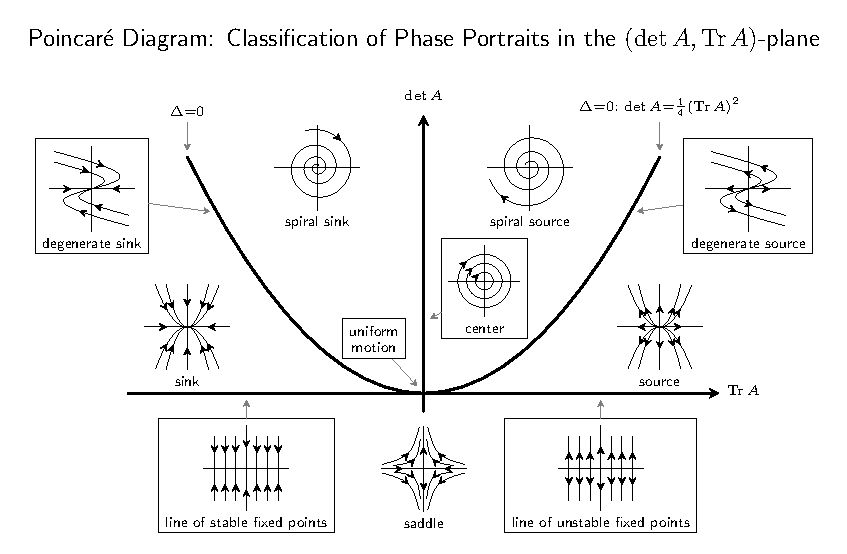
\includegraphics[height=0.7\textheight]{img/examples/poincare.pdf}
    \end{figure}
    \textbf{Source}: {\scriptsize\url{https://texample.net/tikz/examples/poincare/}}
    \\
    \textbf{Size}: 168 lines of code
\end{frame}

\begin{frame}{Showcase - Example \#3}
    \begin{figure}
        \centering
        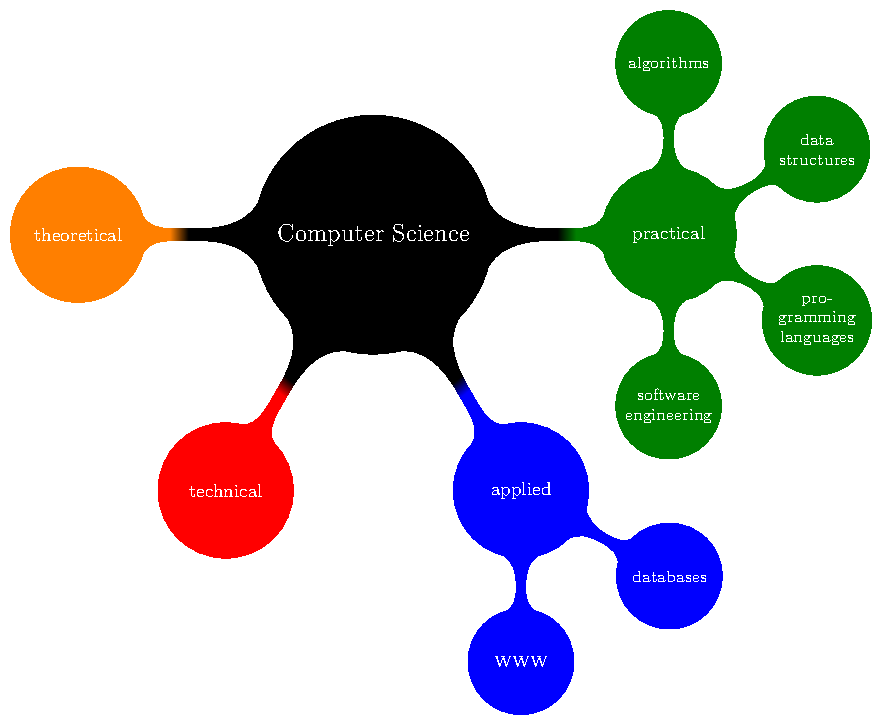
\includegraphics[width=0.6\textwidth]{img/examples/computer-science-mindmap.pdf}
        \caption*{}
        \label{fig:compscimindmap}
    \end{figure}
    \textbf{Source}: {\scriptsize\url{https://texample.net/tikz/examples/computer-science-mindmap/}}
    \\
    \textbf{Size}: 29 lines of code
\end{frame}

\begin{frame}{\TikZ\ - Pros and Cons}
    With \TikZ you get all the \textbf{advantages} of the “\TeX-approach to typesetting” for your graphics:
    \begin{itemize}
        \pro Quick creation of simple graphics
        \pro Precise positioning
        \pro Use of macros
        \pro Often superior typography
        \pro \emph{Code suggestions from CoPilot!}
    \end{itemize}
You also inherit all the \textbf{disadvantages}:
    \begin{itemize}
        \con Steep learning curve
        \con No WYSIWYG
        \con Small changes require a long recompilation time
        \con The code does not really “show” how things will look like
    \end{itemize}
\end{frame}

\begin{frame}{Hello World++: A Picture for Karl’s Students}
    \begin{figure}
        \centering
        \begin{adjustbox}{width=0.9\textwidth}
            \begin{tikzpicture}[
  scale=3, line cap=round,
  % Styles
  axes/.style=,
  important line/.style={very thick},
  information text/.style={rounded corners, fill=red!10, inner sep=1ex}
]
  % Colors
  \colorlet{anglecolor}{green!50!black}
  \colorlet{sincolor}{red}
  \colorlet{tancolor}{orange!80!black}
  \colorlet{coscolor}{blue}
 
  % The graphic
  \draw[help lines,step=0.5cm] (-1.4,-1.4) grid (1.4,1.4);
  \draw (0,0) circle [radius=1cm];
  \begin{scope}[axes]
    \draw[->] (-1.5,0) -- (1.5,0) node[right] {$x$} coordinate(x axis);
    \draw[->] (0,-1.5) -- (0,1.5) node[above] {$y$} coordinate(y axis);
    \foreach \x/\xtext in {-1, -.5/-\frac{1}{2}, 1}
      \draw[xshift=\x cm] (0pt,1pt) -- (0pt,-1pt) node[below,fill=white] {$\xtext$};
    \foreach \y/\ytext in {-1, -.5/-\frac{1}{2}, .5/\frac{1}{2}, 1}
      \draw[yshift=\y cm] (1pt,0pt) -- (-1pt,0pt) node[left,fill=white] {$\ytext$};
  \end{scope}
 
  \filldraw[fill=green!20,draw=anglecolor] (0,0) -- (3mm,0pt) arc [start angle=0, end angle=30, radius=3mm];
  \draw (15:2mm) node[anglecolor] {$\alpha$};
  \draw[important line,sincolor] (30:1cm) -- node[left=1pt,fill=white] {$\sin \alpha$} (30:1cm |- x axis);
  \draw[important line,coscolor] (30:1cm |- x axis) -- node[below=2pt,fill=white] {$\cos \alpha$} (0,0);
  \path [name path=upward line] (1,0) -- (1,1);
  \path [name path=sloped line] (0,0) -- (30:1.5cm);
  \draw [name intersections={of=upward line and sloped line, by=t}]
    [very thick,orange] (1,0) -- node [right=1pt,fill=white]
    {$\displaystyle \tan \alpha \color{black}=\frac{{\color{sincolor}\sin \alpha}}{\color{coscolor}\cos \alpha}$} (t);
  \draw (0,0) -- (t);
  \draw[xshift=1.85cm] node[right,text width=6cm,information text]
  {The {\color{anglecolor} angle $\alpha$} is $30^\circ$ in the example ($\pi/6$ in radians). 
   The {\color{sincolor}sine of $\alpha$}, which is the height of the red line, is
   \[{\color{sincolor} \sin \alpha} = 1/2.\]
   By the Theorem of Pythagoras we have ${\color{coscolor}\cos^2 \alpha} + {\color{sincolor}\sin^2 \alpha} = 1$.
   Thus the length of the blue line, which is the {\color{coscolor} cosine of $\alpha$}, must be
   \[{\color{coscolor}\cos \alpha} = \sqrt{1 - 1/4} = \frac{1}{2}\sqrt{3}.\]
   This shows that ${\color{tancolor}\tan \alpha}$, which is the height of the orange line, is
   \[{\color{tancolor}\tan \alpha} = \frac{{\color{sincolor}\sin \alpha}}{{\color{coscolor}\cos \alpha}} = 1/\sqrt{3}.\]
  };
\end{tikzpicture}
        \end{adjustbox}
    \end{figure}
    \textbf{Source}: {\scriptsize\url{https://texample.net/tikz/examples/tutorial/}}
    \\
    \textbf{Size}: 46 lines of code
\end{frame}

\begin{frame}{Hello World (1) - Drawing}
  \begin{columns}
    \begin{column}{0.35\textwidth}
      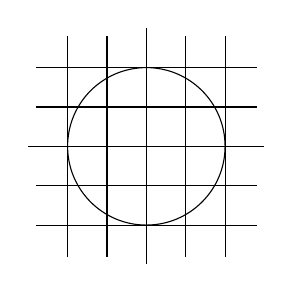
\begin{tikzpicture}
  \draw (-1.5,0) -- (1.5,0);
  \draw (0,-1.5) -- (0,1.5);
  \draw (0,0) circle [radius=1];
  \draw[step=0.5] (-1.4,-1.4) grid (1.4,1.4);
\end{tikzpicture}

    \end{column}
    \begin{column}{0.65\textwidth}
      \inputminted{TeX}{img/tutorial/karl/karl_step_1_standalone.tex}
    \end{column}
  \end{columns}
\end{frame}

\begin{frame}{Hello World (2) - Arguments}
  \begin{columns}
    \begin{column}{0.35\textwidth}
      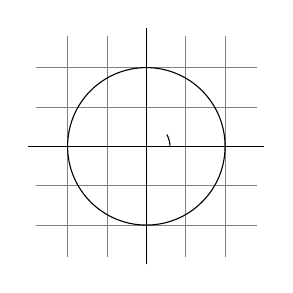
\begin{tikzpicture}
  \draw[step=.5cm,gray,very thin] (-1.4,-1.4) grid (1.4,1.4);
  \draw (-1.5,0) -- (1.5,0);
  \draw (0,-1.5) -- (0,1.5);
  \draw (0,0) circle [radius=1cm];
  \draw (3mm,0mm) arc [start angle=0, end angle=30, radius=3mm];
\end{tikzpicture}

    \end{column}
    \begin{column}{0.65\textwidth}
      \inputminted[firstline=6,lastline=10]{TeX}{img/tutorial/karl/karl_step_2_standalone.tex}
    \end{column}
  \end{columns}
\end{frame}

\begin{frame}{Hello World (3) - Styles}
  \begin{columns}
    \begin{column}{0.35\textwidth}
      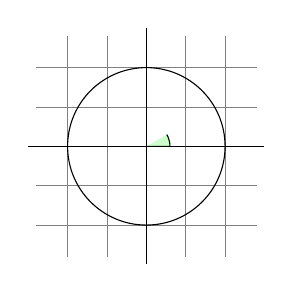
\begin{tikzpicture}[
  help lines/.style={very thin, gray},
]
  \draw[help lines, step=0.5cm] (-1.4,-1.4) grid (1.4,1.4);
  \draw (-1.5,0) -- (1.5,0);
  \draw (0,-1.5) -- (0,1.5);
  \draw (0,0) circle [radius=1cm];
  \filldraw[fill=green!20,draw] (0,0) -- (3mm,0pt) arc [start angle=0, end angle=30, radius=3mm];
\end{tikzpicture}

    \end{column}
    \begin{column}{0.65\textwidth}
      \inputminted[firstline=5,lastline=13]{TeX}{img/tutorial/karl/karl_step_3_standalone.tex}
    \end{column}
  \end{columns}
\end{frame}

\begin{frame}{Hello World++: A Picture for Karl’s Students}
    \inputminted[lastline=26]{TeX}{img/tutorial/karl/karl.tex}
\end{frame}
\begin{frame}{Hello World++: A Picture for Karl’s Students}
    \inputminted[firstline=27]{TeX}{img/tutorial/karl/karl.tex}
\end{frame}

\begin{frame}{\TikZ for Neural Networks}
    \begin{itemize}
        \item A simple MLP
        \item Transformers
        \item Graph Networks
    \end{itemize}
\end{frame}

\begin{frame}{A simple MLP}
  \begin{figure}
    \centering
    \begin{adjustbox}{height=0.88\textheight, center}
      \begin{tikzpicture}[
  inputnode/.style={draw, circle, fill=red!50, inner sep=2pt},
  outnode/.style={draw, circle, fill=orange!50, inner sep=2pt},
  hiddenunit/.style={draw, circle, minimum size=10pt},
  weights/.style={-stealth, thin, opacity=0.8},
]
  \node[inputnode] (x1) {$\mathrm{x}_1$};
  \node[inputnode, above=of x1] (x0) {$\mathrm{x}_0$};
  \node[inputnode, below=of x1] (x2) {$\mathrm{x}_2$};

  \node[hiddenunit, right=of x1] (h2) {};
  \node[hiddenunit, above=of h2] (h1) {};
  \node[hiddenunit, above=of h1] (h0) {};
  \node[hiddenunit, below=of h2] (h3) {};
  \node[hiddenunit, below=of h3] (h4) {};

  \node[outnode, right=of h2] (y0) {$\mathrm{y}$};

  \foreach \x in {x0, x1, x2} {
    \foreach \h in {h0, h1, h2, h3, h4} {
      \draw[weights] (\x) -- (\h);
    }
  }
  \foreach \h in {h0, h1, h2, h3, h4} {
    \foreach \y in {y0} {
      \draw[weights] (\h) -- (\y);
    }
  }
\end{tikzpicture}

    \end{adjustbox}
  \end{figure}
\end{frame}

\begin{frame}{A simple MLP}
  \begin{columns}
    \begin{column}{0.26\textwidth}
      \begin{figure}
        \centering
        \begin{adjustbox}{height=0.48\textheight, center}
          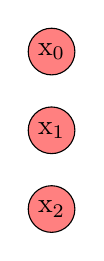
\begin{tikzpicture}[
  inputnode/.style={draw, circle, fill=red!50, inner sep=2pt},
]
  \node[inputnode] (x0) at (0, 1) {$\mathrm{x}_0$};
  \node[inputnode] (x1) at (0, 0) {$\mathrm{x}_1$};
  \node[inputnode] (x2) at (0, -1) {$\mathrm{x}_2$};
\end{tikzpicture}

        \end{adjustbox}
      \end{figure}
    \end{column}
    \begin{column}{0.74\textwidth}
      \inputminted[]{TeX}{img/tutorial/mlp/mlp_step_1.tex}
    \end{column}
  \end{columns}
\end{frame}

\begin{frame}{A simple MLP}
  \begin{columns}
    \begin{column}{0.26\textwidth}
      \begin{figure}
        \centering
        \begin{adjustbox}{height=0.48\textheight, center}
          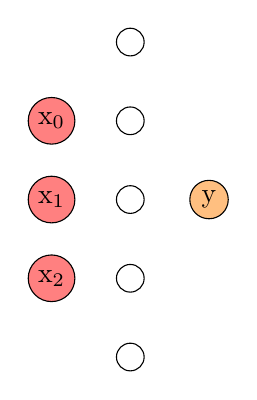
\begin{tikzpicture}[
  inputnode/.style={draw, circle, fill=red!50, inner sep=2pt},
  hiddenunit/.style={draw, circle, minimum size=10pt},
  outnode/.style={draw, circle, fill=orange!50, inner sep=2pt},
]
  \node[inputnode] (x0) at (0, 1) {$\mathrm{x}_0$};
  \node[inputnode] (x1) at (0, 0) {$\mathrm{x}_1$};
  \node[inputnode] (x2) at (0, -1) {$\mathrm{x}_2$};

  \node[hiddenunit] (h2) at (1, 2) {};
  \node[hiddenunit] (h1) at (1, 1) {};
  \node[hiddenunit] (h0) at (1, 0) {};
  \node[hiddenunit] (h3) at (1, -1) {};
  \node[hiddenunit] (h4) at (1, -2) {};

  \node[outnode] (y0) at (2, 0) {$\mathrm{y}$};
\end{tikzpicture}


        \end{adjustbox}
      \end{figure}
    \end{column}
    \begin{column}{0.74\textwidth}
      \inputminted[]{TeX}{img/tutorial/mlp/mlp_step_2.tex}
    \end{column}
  \end{columns}
\end{frame}

\begin{frame}{A simple MLP}
  \begin{columns}
    \begin{column}{0.26\textwidth}
      \begin{figure}
        \centering
        \begin{adjustbox}{width=0.98\textwidth, center}
          \begin{tikzpicture}[
  inputnode/.style={draw, circle, fill=red!50, inner sep=2pt},
  outnode/.style={draw, circle, fill=orange!50, inner sep=2pt},
  hiddenunit/.style={draw, circle, minimum size=10pt},
  weights/.style={-stealth, thin, opacity=0.8},
]
  \node[inputnode] (x1) {$\mathrm{x}_1$};
  \node[inputnode, above=of x1] (x0) {$\mathrm{x}_0$};
  \node[inputnode, below=of x1] (x2) {$\mathrm{x}_2$};

  \node[hiddenunit, right=of x1] (h2) {};
  \node[hiddenunit, above=of h2] (h1) {};
  \node[hiddenunit, above=of h1] (h0) {};
  \node[hiddenunit, below=of h2] (h3) {};
  \node[hiddenunit, below=of h3] (h4) {};

  \node[outnode, right=of h2] (y0) {$\mathrm{y}$};

  \foreach \x in {x0, x1, x2} {
    \foreach \h in {h0, h1, h2, h3, h4} {
      \draw[weights] (\x) -- (\h);
    }
  }
  \foreach \h in {h0, h1, h2, h3, h4} {
    \foreach \y in {y0} {
      \draw[weights] (\h) -- (\y);
    }
  }
\end{tikzpicture}

        \end{adjustbox}
      \end{figure}
    \end{column}
    \begin{column}{0.74\textwidth}
      \inputminted[]{TeX}{img/tutorial/mlp/mlp.tex}
    \end{column}
  \end{columns}
\end{frame}

\begin{frame}{\sout{Attention}\TikZ Is All You Need}
  \begin{figure}
    \centering
    \resizebox{!}{0.9\textheight}{%
      \begin{tikzpicture}[
  module/.style={draw, very thick, rounded corners, minimum width=15ex},
  embmodule/.style={module, fill=red!20},
  mhamodule/.style={module, fill=orange!20},
  lnmodule/.style={module, fill=yellow!20},
  ffnmodule/.style={module, fill=cyan!20},
  arrow/.style={-stealth', thick, rounded corners},
]

  \node (inputs) {Inputs};
  \node[above=of inputs, embmodule, align=center] (inputemb) {Input\\Embedding};
  \node[above=of inputemb, draw, thick, circle] (embplus) {$+$};
  \node[left=of embplus, draw, thick, circle, inner sep=0pt,label={[align=left]left:Positional\\Encoding}] (pe) {\tikz \draw[scale=0.1] plot[domain=0.0:6.28] (\x,{sin(\x r)});};

  \node[above=of embplus, mhamodule, align=center] (mha) {Multi-Head\\Attention};
  \node[above=of mha, lnmodule, align=center] (addnorm1) {Add \& Norm};
  \node[above=of addnorm1, ffnmodule, align=center] (ffn) {Feed\\Forward};
  \node[above=of ffn, lnmodule, align=center] (addnorm2) {Add \& Norm};
  \node[above=of addnorm2] (outputs) {Outputs};

  \coordinate (mharesidual) at ($(mha.south)!0.5!(embplus.north)$);
  \coordinate (ffnresidual) at ($(ffn.south)!0.5!(addnorm1.north)$);
  \coordinate (mhafork) at ($(mha.south)!0.5!(mharesidual)$);
  \coordinate[left=of addnorm1] (ln1residualleft);
  \coordinate[left=of addnorm2] (ln2residualleft);

  \node[fit={(mha)(addnorm2)(mharesidual)(ln1residualleft)}, draw, ultra thick, rounded corners, label=left:$\mathrm{N\times}$] (encoder) {};

  \draw[arrow] (inputs) -- (inputemb);
  \draw[arrow] (inputemb) -- (embplus);
  \draw[arrow] (pe) -- (embplus);
  \draw[arrow] (embplus) -- (mha);
  \draw[arrow] (mha) -- (addnorm1);
  \draw[arrow] (addnorm1) -- (ffn);
  \draw[arrow] (ffn) -- (addnorm2);
  \draw[arrow] (addnorm2) -- (outputs);

  \draw[arrow] (mharesidual)-|(ln1residualleft)--(addnorm1);
  \draw[arrow] (ffnresidual)-|(ln2residualleft)--(addnorm2);
  \draw[arrow] (mhafork)-|($(mha.south)!0.5!(mha.south west)$);
  \draw[arrow] (mhafork)-|($(mha.south)!0.5!(mha.south east)$);
\end{tikzpicture}

  % \node[left=of embplus, draw, thick, circle, label={[align=left]left:Positional\\Encoding}] (pe) {\tikz \draw[scale=0.05] plot[domain=0.0:6.28] function {sin(x)};};

    }
  \end{figure}
\end{frame}

\begin{frame}{\sout{Attention}\TikZ Is All You Need}
\begin{columns}
  \begin{column}{0.4\textwidth}
    \begin{figure}
      \centering
      \resizebox{!}{0.9\textheight}{%
        \begin{tikzpicture}[
  module/.style={draw, very thick, rounded corners, minimum width=15ex},
  embmodule/.style={module, fill=red!20},
  mhamodule/.style={module, fill=orange!20},
  lnmodule/.style={module, fill=yellow!20},
  ffnmodule/.style={module, fill=cyan!20},
  arrow/.style={-stealth', thick, rounded corners},
]
  \node (inputs) {Inputs};
  \node[above=of inputs, embmodule, align=center] (inputemb) {Input\\Embedding};
  \node[above=of inputemb, draw, thick, circle] (embplus) {$+$};
  \node[above=of embplus, mhamodule, align=center] (mha) {Multi-Head\\Attention};
  \node[above=of mha, lnmodule, align=center] (addnorm1) {Add \& Norm};
  \node[above=of addnorm1, ffnmodule, align=center] (ffn) {Feed\\Forward};
  \node[above=of ffn, lnmodule, align=center] (addnorm2) {Add \& Norm};
  \node[above=of addnorm2] (outputs) {Outputs};
\end{tikzpicture}


      }
    \end{figure}
  \end{column}
  \begin{column}{0.7\textwidth}
    \inputminted[]{TeX}{img/tutorial/transformers/transformers_step_1.tex}
  \end{column}
\end{columns}
\end{frame}

\begin{frame}{\sout{Attention}\TikZ Is All You Need}
\begin{columns}
  \begin{column}{0.4\textwidth}
    \begin{figure}
      \centering
      \resizebox{!}{0.9\textheight}{%
        \begin{tikzpicture}[
  module/.style={draw, very thick, rounded corners, minimum width=15ex},
  embmodule/.style={module, fill=red!20},
  mhamodule/.style={module, fill=orange!20},
  lnmodule/.style={module, fill=yellow!20},
  ffnmodule/.style={module, fill=cyan!20},
  arrow/.style={-stealth', thick, rounded corners},
]

  \node (inputs) {Inputs};
  \node[above=of inputs, embmodule, align=center] (inputemb) {Input\\Embedding};
  \node[above=of inputemb, draw, thick, circle] (embplus) {$+$};
  \node[left=of embplus, draw, thick, circle, inner sep=0pt,label={[align=left]left:Positional\\Encoding}] (pe) {\tikz \draw[scale=0.1] plot[domain=0.0:6.28] (\x,{sin(\x r)});};

  \node[above=of embplus, mhamodule, align=center] (mha) {Multi-Head\\Attention};
  \node[above=of mha, lnmodule, align=center] (addnorm1) {Add \& Norm};
  \node[above=of addnorm1, ffnmodule, align=center] (ffn) {Feed\\Forward};
  \node[above=of ffn, lnmodule, align=center] (addnorm2) {Add \& Norm};
  \node[above=of addnorm2] (outputs) {Outputs};

  \draw[arrow] (inputs) -- (inputemb);
  \draw[arrow] (inputemb) -- (embplus);
  \draw[arrow] (pe) -- (embplus);
  \draw[arrow] (embplus) -- (mha);
  \draw[arrow] (mha) -- (addnorm1);
  \draw[arrow] (addnorm1) -- (ffn);
  \draw[arrow] (ffn) -- (addnorm2);
  \draw[arrow] (addnorm2) -- (outputs);
\end{tikzpicture}


      }
    \end{figure}
  \end{column}
  \begin{column}{0.7\textwidth}
    \inputminted[firstline=7,lastline=7]{TeX}{img/tutorial/transformers/transformers.tex}
    {\tikz \node[inner ysep=0pt] (dots) {$\vdots$};}
    \inputminted[firstline=13,lastline=13]{TeX}{img/tutorial/transformers/transformers.tex}
    {\tikz \node[inner ysep=0pt] (dots) {$\vdots$};}
    \inputminted[firstline=29,lastline=36]{TeX}{img/tutorial/transformers/transformers.tex}
  \end{column}
\end{columns}
\end{frame}

\begin{frame}{\sout{Attention}\TikZ Is All You Need}
\begin{columns}
  \begin{column}{0.4\textwidth}
    \begin{figure}
      \centering
      \resizebox{!}{0.9\textheight}{%
        \begin{tikzpicture}[
  module/.style={draw, very thick, rounded corners, minimum width=15ex},
  embmodule/.style={module, fill=red!20},
  mhamodule/.style={module, fill=orange!20},
  lnmodule/.style={module, fill=yellow!20},
  ffnmodule/.style={module, fill=cyan!20},
  arrow/.style={-stealth', thick, rounded corners},
]

  \node (inputs) {Inputs};
  \node[above=of inputs, embmodule, align=center] (inputemb) {Input\\Embedding};
  \node[above=of inputemb, draw, thick, circle] (embplus) {$+$};
  \node[left=of embplus, draw, thick, circle, inner sep=0pt,label={[align=left]left:Positional\\Encoding}] (pe) {\tikz \draw[scale=0.1] plot[domain=0.0:6.28] (\x,{sin(\x r)});};

  \node[above=of embplus, mhamodule, align=center] (mha) {Multi-Head\\Attention};
  \node[above=of mha, lnmodule, align=center] (addnorm1) {Add \& Norm};
  \node[above=of addnorm1, ffnmodule, align=center] (ffn) {Feed\\Forward};
  \node[above=of ffn, lnmodule, align=center] (addnorm2) {Add \& Norm};
  \node[above=of addnorm2] (outputs) {Outputs};

  \draw[arrow] (inputs) -- (inputemb);
  \draw[arrow] (inputemb) -- (embplus);
  \draw[arrow] (pe) -- (embplus);
  \draw[arrow] (embplus) -- (mha);
  \draw[arrow] (mha) -- (addnorm1);
  \draw[arrow] (addnorm1) -- (ffn);
  \draw[arrow] (ffn) -- (addnorm2);
  \draw[arrow] (addnorm2) -- (outputs);
\end{tikzpicture}


      }
    \end{figure}
  \end{column}
  \begin{column}{0.7\textwidth}
    \inputminted[firstline=7,lastline=7]{TeX}{img/tutorial/transformers/transformers.tex}
    \begin{tikzpicture}
      \node[inner ysep=0pt] (dots) {$\vdots$};
      \node[right=of dots,yshift=-2pt,inner ysep=0pt, red!80] (dots2) {\scriptsize This is inline \TikZ!};
      \draw[-Straight Barb, thick, red!80] (dots2) -- (dots.east|-dots2);
    \end{tikzpicture}
    \inputminted[firstline=13,lastline=13]{TeX}{img/tutorial/transformers/transformers.tex}
    \begin{tikzpicture}
      \node[inner ysep=0pt] (dots) {$\vdots$};
      \node[right=of dots,yshift=-2pt,inner ysep=0pt, red!80] (dots2) {\scriptsize This is inline \TikZ!};
      \draw[-Straight Barb, thick, red!80] (dots2) -- (dots.east|-dots2);
    \end{tikzpicture}
    \inputminted[firstline=29,lastline=36]{TeX}{img/tutorial/transformers/transformers.tex}
  \end{column}
\end{columns}
\end{frame}

\begin{frame}{\sout{Attention}\TikZ Is All You Need}
\begin{columns}
  \begin{column}{0.4\textwidth}
    \begin{figure}
      \centering
      \resizebox{!}{0.9\textheight}{%
        \begin{tikzpicture}[
  module/.style={draw, very thick, rounded corners, minimum width=15ex},
  embmodule/.style={module, fill=red!20},
  mhamodule/.style={module, fill=orange!20},
  lnmodule/.style={module, fill=yellow!20},
  ffnmodule/.style={module, fill=cyan!20},
  arrow/.style={-stealth', thick, rounded corners},
]

  \node (inputs) {Inputs};
  \node[above=of inputs, embmodule, align=center] (inputemb) {Input\\Embedding};
  \node[above=of inputemb, draw, thick, circle] (embplus) {$+$};
  \node[left=of embplus, draw, thick, circle, inner sep=0pt,label={[align=left]left:Positional\\Encoding}] (pe) {\tikz \draw[scale=0.1] plot[domain=0.0:6.28] (\x,{sin(\x r)});};

  \node[above=of embplus, mhamodule, align=center] (mha) {Multi-Head\\Attention};
  \node[above=of mha, lnmodule, align=center] (addnorm1) {Add \& Norm};
  \node[above=of addnorm1, ffnmodule, align=center] (ffn) {Feed\\Forward};
  \node[above=of ffn, lnmodule, align=center] (addnorm2) {Add \& Norm};
  \node[above=of addnorm2] (outputs) {Outputs};

  \coordinate (mharesidual) at ($(mha.south)!0.5!(embplus.north)$);
  \coordinate (ffnresidual) at ($(ffn.south)!0.5!(addnorm1.north)$);
  \coordinate (mhafork) at ($(mha.south)!0.5!(mharesidual)$);
  \coordinate[left=of addnorm1] (ln1residualleft);
  \coordinate[left=of addnorm2] (ln2residualleft);

  \node[fit={(mha)(addnorm2)(mharesidual)(ln1residualleft)}, draw, ultra thick, rounded corners, label=left:$\mathrm{N\times}$] (encoder) {};

  \draw[arrow] (inputs) -- (inputemb);
  \draw[arrow] (inputemb) -- (embplus);
  \draw[arrow] (pe) -- (embplus);
  \draw[arrow] (embplus) -- (mha);
  \draw[arrow] (mha) -- (addnorm1);
  \draw[arrow] (addnorm1) -- (ffn);
  \draw[arrow] (ffn) -- (addnorm2);
  \draw[arrow] (addnorm2) -- (outputs);

  \draw[arrow] (mharesidual)-|(ln1residualleft)--(addnorm1);
  \draw[arrow] (ffnresidual)-|(ln2residualleft)--(addnorm2);
  \draw[arrow] (mhafork)-|($(mha.south)!0.5!(mha.south west)$);
  \draw[arrow] (mhafork)-|($(mha.south)!0.5!(mha.south east)$);
\end{tikzpicture}

  % \node[left=of embplus, draw, thick, circle, label={[align=left]left:Positional\\Encoding}] (pe) {\tikz \draw[scale=0.05] plot[domain=0.0:6.28] function {sin(x)};};

      }
    \end{figure}
  \end{column}
  \begin{column}{0.7\textwidth}
    \inputminted[firstline=21,lastline=25]{TeX}{img/tutorial/transformers/transformers.tex}
    {\tikz \node[inner ysep=0pt] (dots) {$\vdots$};}
    \inputminted[firstline=27,lastline=27]{TeX}{img/tutorial/transformers/transformers.tex}
    {\tikz \node[inner ysep=0pt] (dots) {$\vdots$};}
    \inputminted[firstline=38,lastline=41]{TeX}{img/tutorial/transformers/transformers.tex}
  \end{column}
\end{columns}
\end{frame}

\begin{frame}{\sout{Attention}\TikZ Is All You Need}
  \begin{figure}
    \centering
    \resizebox{!}{0.9\textheight}{%
      \begin{tikzpicture}[
  module/.style={draw, very thick, rounded corners, minimum width=15ex},
  embmodule/.style={module, fill=red!20},
  mhamodule/.style={module, fill=orange!20},
  lnmodule/.style={module, fill=yellow!20},
  ffnmodule/.style={module, fill=cyan!20},
  arrow/.style={-stealth', thick, rounded corners},
]

  \node (inputs) {Inputs};
  \node[above=of inputs, embmodule, align=center] (inputemb) {Input\\Embedding};
  \node[above=of inputemb, draw, thick, circle] (embplus) {$+$};
  \node[left=of embplus, draw, thick, circle, inner sep=0pt,label={[align=left]left:Positional\\Encoding}] (pe) {\tikz \draw[scale=0.1] plot[domain=0.0:6.28] (\x,{sin(\x r)});};

  \node[above=of embplus, mhamodule, align=center] (mha) {Multi-Head\\Attention};
  \node[above=of mha, lnmodule, align=center] (addnorm1) {Add \& Norm};
  \node[above=of addnorm1, ffnmodule, align=center] (ffn) {Feed\\Forward};
  \node[above=of ffn, lnmodule, align=center] (addnorm2) {Add \& Norm};
  \node[above=of addnorm2] (outputs) {Outputs};

  \coordinate (mharesidual) at ($(mha.south)!0.5!(embplus.north)$);
  \coordinate (ffnresidual) at ($(ffn.south)!0.5!(addnorm1.north)$);
  \coordinate (mhafork) at ($(mha.south)!0.5!(mharesidual)$);
  \coordinate[left=of addnorm1] (ln1residualleft);
  \coordinate[left=of addnorm2] (ln2residualleft);

  \node[fit={(mha)(addnorm2)(mharesidual)(ln1residualleft)}, draw, ultra thick, rounded corners, label=left:$\mathrm{N\times}$] (encoder) {};

  \draw[arrow] (inputs) -- (inputemb);
  \draw[arrow] (inputemb) -- (embplus);
  \draw[arrow] (pe) -- (embplus);
  \draw[arrow] (embplus) -- (mha);
  \draw[arrow] (mha) -- (addnorm1);
  \draw[arrow] (addnorm1) -- (ffn);
  \draw[arrow] (ffn) -- (addnorm2);
  \draw[arrow] (addnorm2) -- (outputs);

  \draw[arrow] (mharesidual)-|(ln1residualleft)--(addnorm1);
  \draw[arrow] (ffnresidual)-|(ln2residualleft)--(addnorm2);
  \draw[arrow] (mhafork)-|($(mha.south)!0.5!(mha.south west)$);
  \draw[arrow] (mhafork)-|($(mha.south)!0.5!(mha.south east)$);
\end{tikzpicture}

  % \node[left=of embplus, draw, thick, circle, label={[align=left]left:Positional\\Encoding}] (pe) {\tikz \draw[scale=0.05] plot[domain=0.0:6.28] function {sin(x)};};

    }
  \end{figure}
\end{frame}

\begin{frame}{Graph Network Flavours}
    \begin{figure}
        \centering
        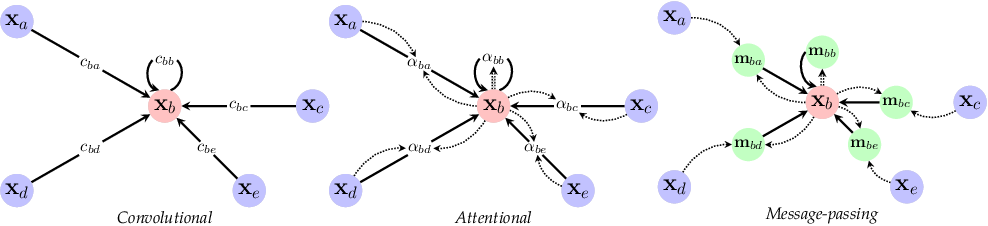
\includegraphics[width=0.9\textwidth]{./img/tutorial/gnn/82-Figure17-1.png}
    \end{figure}
\end{frame}

\begin{frame}[t]{Final notes}
    \begin{itemize}
        \item You can use \TikZ inline!
        \item You can export Matplotlib to pgf!
          \begin{itemize}
            \item \url{https://matplotlib.org/stable/tutorials/text/pgf.html}
          \end{itemize}
        \item Same with programming: Learn-by-doing!
    \end{itemize}
    \tikz[overlay] \draw[scale=0.3,domain=-6.28:6.28,smooth,samples=201,variable=\t] plot ({30+\t*sin(\t r)},{-4+\t*cos(\t r)})
      node[label={[red!80]right:Inline \TikZ}] () {};
\end{frame}

\begin{frame}{Personal portfolio collage}
  \begin{figure}
    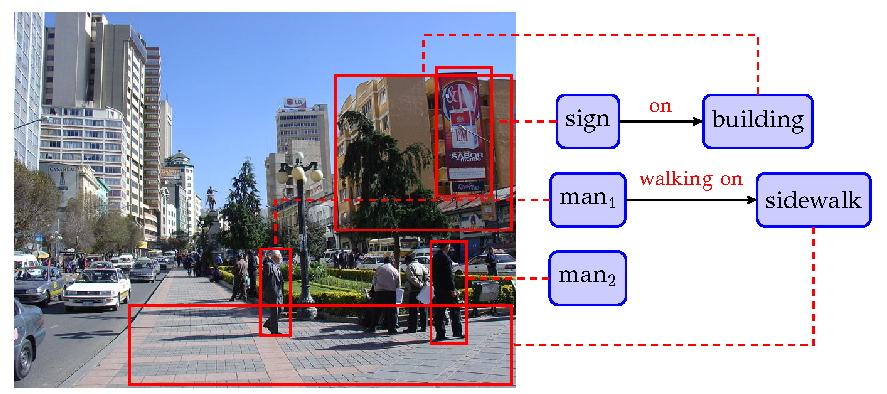
\includegraphics[width=0.98\textwidth]{./img/portfolio/scene_graph_generation.pdf}
  \end{figure}
\end{frame}

\begin{frame}{Personal portfolio collage}
  \begin{figure}
    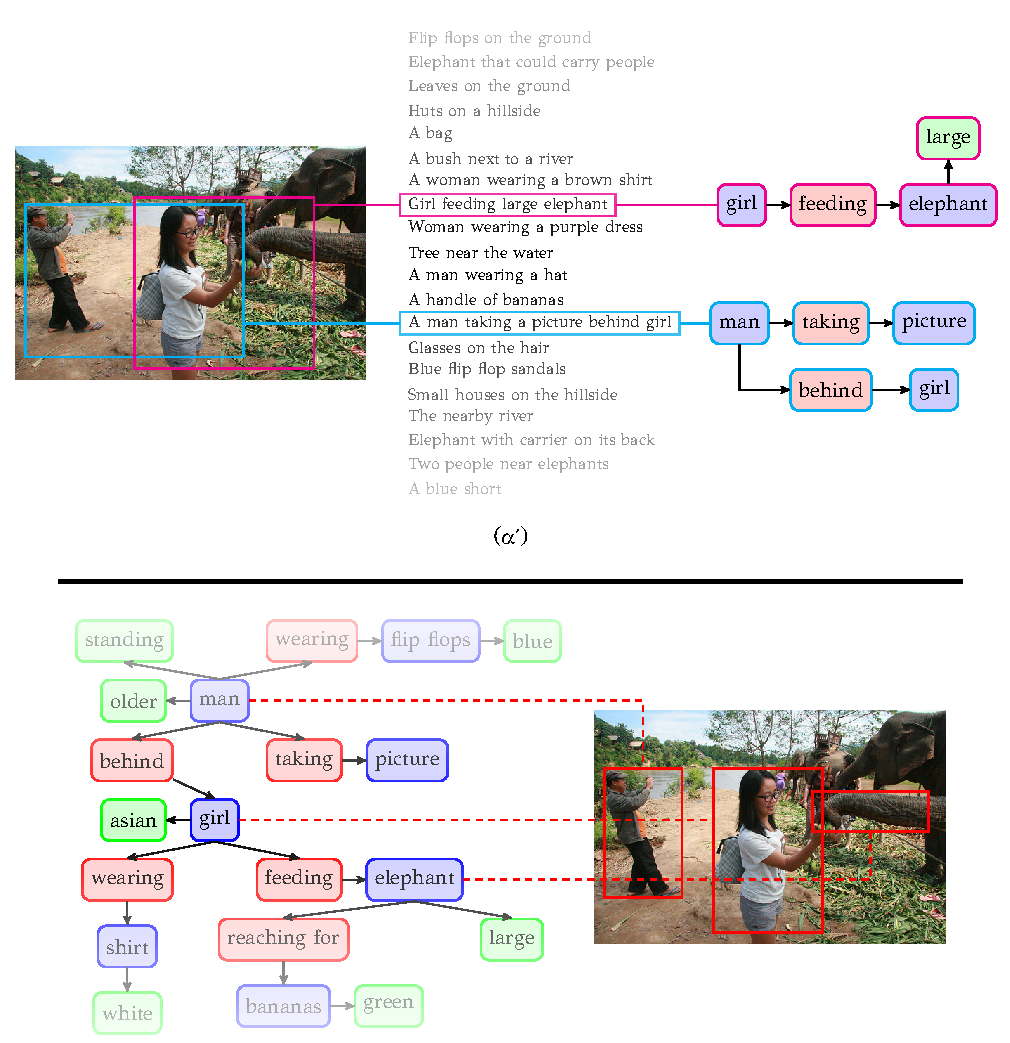
\includegraphics[height=0.9\textheight]{./img/portfolio/visual_genome_1.pdf}
  \end{figure}
\end{frame}

\begin{frame}{Personal portfolio collage}
  \begin{figure}
    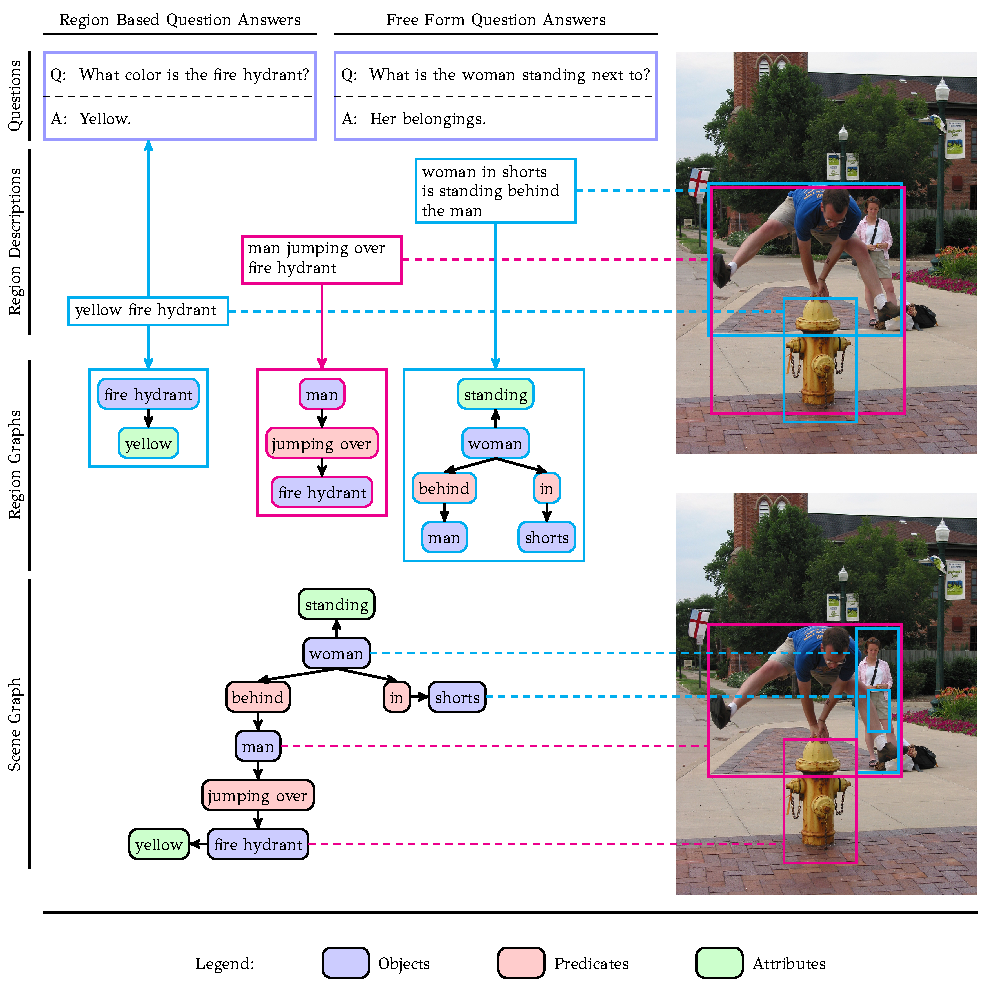
\includegraphics[height=0.9\textheight]{./img/portfolio/visual_genome_2.pdf}
  \end{figure}
\end{frame}

\begin{frame}{Personal portfolio collage}
  \begin{figure}
    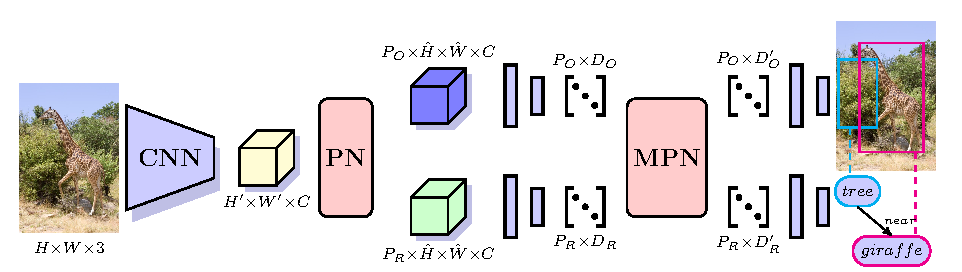
\includegraphics[width=0.98\textwidth]{./img/portfolio/model_architecture.pdf}
  \end{figure}
\end{frame}

\begin{frame}{Personal portfolio collage}
  \begin{figure}
    \resizebox{!}{0.9\textheight}{%
      \begin{tikzpicture}[scale=.4,every node/.style={minimum size=1cm}, on grid, line join=round]
  \begin{scope}[
      every node/.append style={yslant=-0.6}, yslant=-0.6]

    \coordinate (L1) at (2,1);
    \coordinate (L2) at ($ (L1)+(4,-3) $);
    \coordinate (L3) at ($ (L1)+(3,-3) $);
    \coordinate (L4) at ($ (L2)+(-3,3) $);
    \coordinate (L5) at ($ (L1)+(-4,-4) $);

    \fill[blue!40, opacity=.9] (L1) rectangle (L2);

    \only<1>\filldraw[fill=blue!60, draw=black, thick, opacity=.9] (L1) rectangle (L3);
    \only<3>\filldraw[fill=blue!60, draw=black, thick, opacity=.9] (L2) rectangle (L4);

    \draw[black, very thick] (L1) rectangle (L2);
    \draw[black, thin] (L1) grid (L2);
  \end{scope}

  \begin{scope}[
      every node/.append style={yslant=0.4}, yslant=0.4]

    \coordinate (R1) at (6,-5);
    \coordinate (R2) at ($ (R1)+(4,-3) $);
    \coordinate (R3) at ($ (R1)+(3,-3) $);
    \coordinate (R4) at ($ (R2)+(-3,3) $);
    \coordinate (R5) at ($ (R2)+(2,-1) $);
    \coordinate (R6) at ($ (R1)+(-1,-4) $);

    \fill[blue!40, opacity=.9] (R1) rectangle (R2);

    \only<3>\filldraw[fill=blue!60, draw=black, thick, opacity=.9] (R1) rectangle (R3);
    \only<4>\filldraw[fill=blue!60, draw=black, thick, opacity=.9] (R2) rectangle (R4);

    \draw[black, very thick] (R1) rectangle (R2);
    \draw[black, thin] (R1) grid (R2);
  \end{scope}

  \begin{scope}[
      every node/.append style={yslant=-0.6,xslant=1.0},
      yslant=-0.6,xslant=1.0]

    \coordinate (IA) at (1,1);
    \coordinate (IB) at (1,4);
    \coordinate (IC) at (4,1);
    \coordinate (ID) at (4,4);
    \coordinate (IE) at (1,2);
    \coordinate (IF) at (1,5);
    \coordinate (IG) at (4,2);
    \coordinate (IH) at (4,5);
    \coordinate (II) at (2,1);
    \coordinate (IJ) at (2,4);
    \coordinate (IK) at (5,1);
    \coordinate (IL) at (5,4);
    \coordinate (IM) at (2,2);
    \coordinate (IN) at (2,5);
    \coordinate (IO) at (5,2);
    \coordinate (IP) at (5,5);

    \coordinate (I1) at (0,0);
    \coordinate (I2) at (6,6);
    \coordinate (I3) at (0,6);
    \coordinate (I4) at (6,0);

    \fill[blue!40, opacity=.9] (IA) rectangle (IP);

    \only<1>\filldraw[fill=blue!60, draw=black, thick, opacity=.9] (IA) rectangle (ID);
    \only<2>\filldraw[fill=blue!60, draw=black, thick, opacity=.9] (IE) rectangle (IH);
    \only<3>\filldraw[fill=blue!60, draw=black, thick, opacity=.9] (II) rectangle (IL);
    \only<4>\filldraw[fill=blue!60, draw=black, thick, opacity=.9] (IM) rectangle (IP);

    \draw[black, very thick] (IA) rectangle (IP);
    \draw[black, thin] (IA) grid (IP);
    % \draw[black, dashed] (I1) -- (I3) -- (I2) -- (R5) -- (R6) -- (L5);
  \end{scope}

  \begin{scope}[
      yshift=170,
      every node/.append style={yslant=-0.6,xslant=1.0},
      yslant=-0.6,xslant=1.0]

    \coordinate (OA) at (2,2);
    \coordinate (OB) at (2,3);
    \coordinate (OC) at (3,2);
    \coordinate (OD) at (3,3);
    \coordinate (OE) at (2,3);
    \coordinate (OF) at (2,4);
    \coordinate (OG) at (3,3);
    \coordinate (OH) at (3,4);
    \coordinate (OI) at (3,2);
    \coordinate (OJ) at (3,3);
    \coordinate (OK) at (4,2);
    \coordinate (OL) at (4,3);
    \coordinate (OM) at (3,3);
    \coordinate (ON) at (3,4);
    \coordinate (OO) at (4,3);
    \coordinate (OP) at (4,4);

    \coordinate (O1) at (1,1);
    \coordinate (O2) at (5,5);
    \coordinate (O3) at (1,5);
    \coordinate (O4) at (5,1);

    % \coordinate (Q) at (intersection of IA--OA and I1--I3);
    % \coordinate (R) at (intersection of IA--OA and O1--O4);
    % \only<1>\draw[opacity=0.2] (IA) -- (Q) (IB) -- (Q);
    % \only<1>\draw[opacity=0.5] (Q) -- (R);
    % \only<1>\draw[opacity=0.2] (R) -- (OA);

    \only<1>\draw[opacity=0.5] (IA) -- (OA) (IB) -- (OB) (IC) -- (OC) (ID) -- (OD);
    \only<2>\draw[opacity=0.5] (IE) -- (OE) (IF) -- (OF) (IG) -- (OG) (IH) -- (OH);
    \only<3>\draw[opacity=0.5] (II) -- (OI) (IJ) -- (OJ) (IK) -- (OK) (IL) -- (OL);
    \only<4>\draw[opacity=0.5] (IM) -- (OM) (IN) -- (ON) (IO) -- (OO) (IP) -- (OP);

    \fill[green!80!blue, opacity=.9] (OA) rectangle (OP);

    \only<1>\filldraw[fill=green!60!blue, draw=black, thick, opacity=.9] (OA) rectangle (OD);
    \only<2>\filldraw[fill=green!60!blue, draw=black, thick, opacity=.9] (OB) rectangle (OH);
    \only<3>\filldraw[fill=green!60!blue, draw=black, thick, opacity=.9] (OI) rectangle (OL);
    \only<4>\filldraw[fill=green!60!blue, draw=black, thick, opacity=.9] (OM) rectangle (OP);

    \draw[black, very thick] (OA) rectangle (OP);
    \draw[black, thin] (OA) grid (OP);
    \draw[black, dashed] (O1) rectangle (O2);
  \end{scope}

  \begin{scope}[
      every node/.append style={yslant=-0.6,xslant=1.2},
      yslant=-0.6,xslant=1.2]

    % \filldraw[fill=white, draw=black, dashed, opacity=.6] (I1) rectangle (I2);
    % \filldraw[fill=white, draw=black, dashed, opacity=.6] (O1) rectangle (O2);
  \end{scope}
\end{tikzpicture}
\endinput

    }
  \end{figure}
\end{frame}

\begin{frame}{Personal portfolio collage}
  \begin{figure}
    \centering
    \tikz[remember picture]{\node[inner sep=0pt](rotinput){
    \movie[height = 0.7\textwidth, width = 0.762\textwidth, open]
      {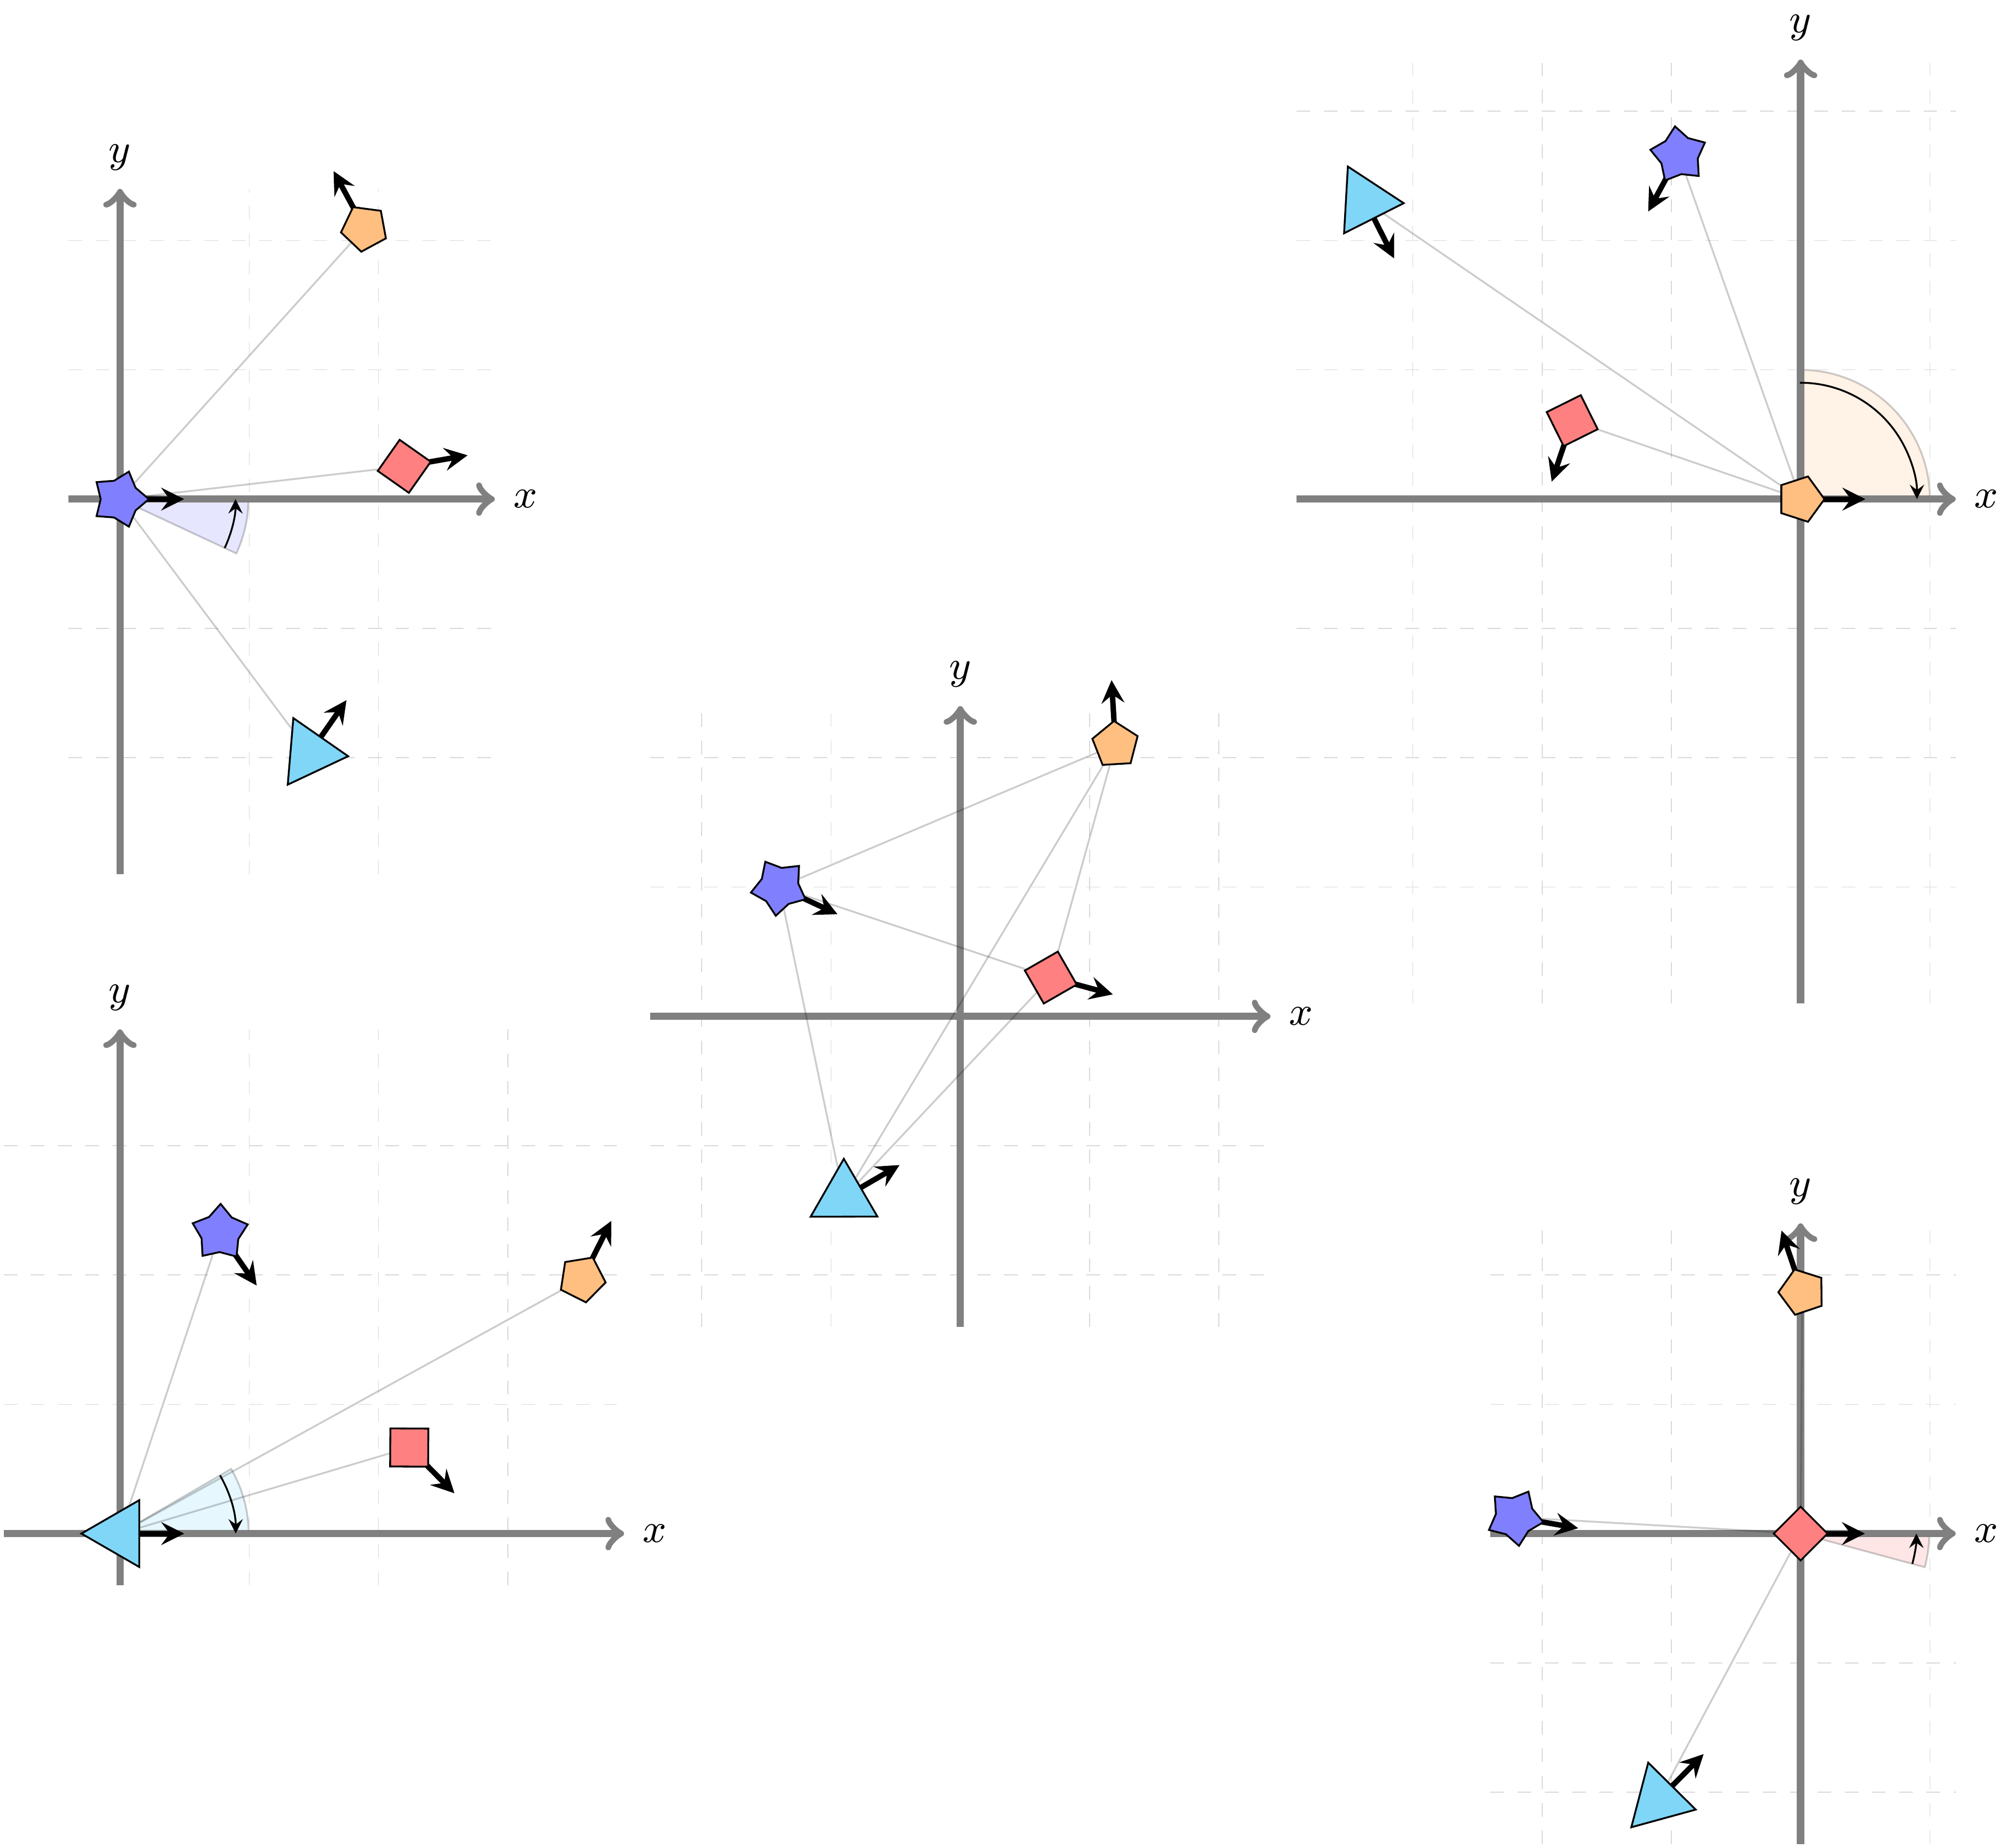
\includegraphics[height = 0.7\textwidth, width=0.762\textwidth]{./img/portfolio/locs_roto.png}}
      {../img/portfolio/locs_roto.mp4}
    }}
  \end{figure}
\end{frame}

\endinput
